% Created by tikzDevice version 0.12 on 2019-01-21 17:17:26
% !TEX encoding = UTF-8 Unicode
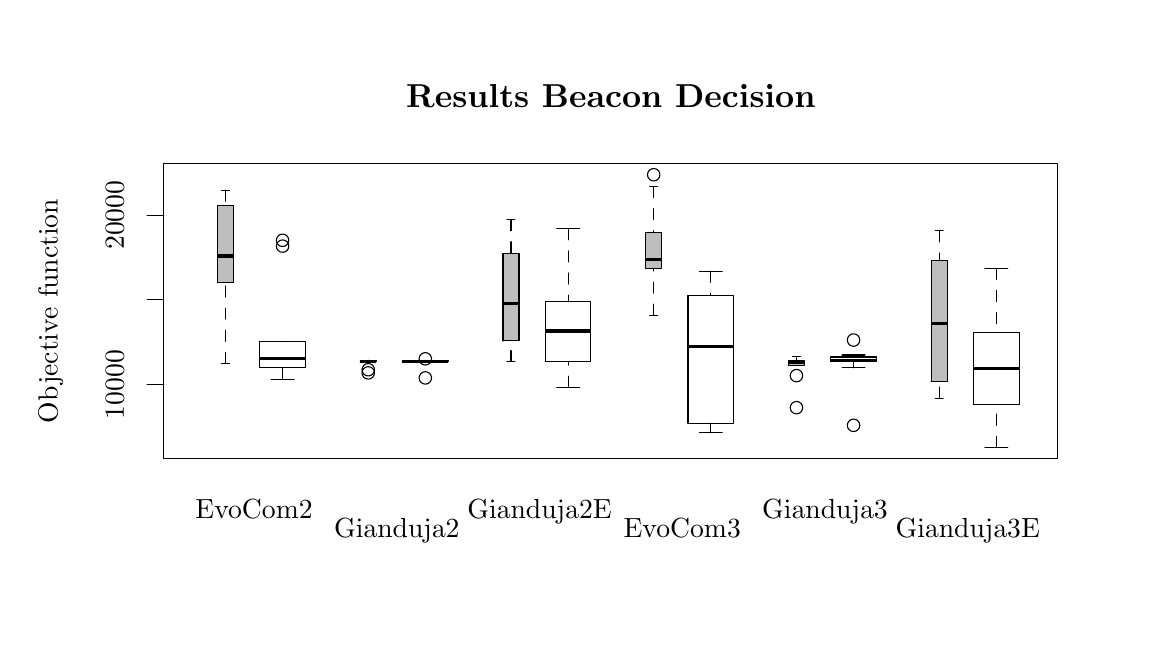
\begin{tikzpicture}[x=1pt,y=1pt]
\definecolor{fillColor}{RGB}{255,255,255}
\path[use as bounding box,fill=fillColor,fill opacity=0.00] (0,0) rectangle (397.48,216.81);
\begin{scope}
\path[clip] ( 49.20, 61.20) rectangle (372.28,167.61);
\definecolor{fillColor}{RGB}{190,190,190}

\path[fill=fillColor] ( 68.59,124.62) --
	( 74.37,124.62) --
	( 74.37,152.52) --
	( 68.59,152.52) --
	cycle;
\definecolor{drawColor}{RGB}{0,0,0}

\path[draw=drawColor,line width= 1.2pt,line join=round] ( 68.59,134.33) -- ( 74.37,134.33);

\path[draw=drawColor,line width= 0.4pt,dash pattern=on 4pt off 4pt ,line join=round,line cap=round] ( 71.48, 95.48) -- ( 71.48,124.62);

\path[draw=drawColor,line width= 0.4pt,dash pattern=on 4pt off 4pt ,line join=round,line cap=round] ( 71.48,158.07) -- ( 71.48,152.52);

\path[draw=drawColor,line width= 0.4pt,line join=round,line cap=round] ( 70.04, 95.48) -- ( 72.93, 95.48);

\path[draw=drawColor,line width= 0.4pt,line join=round,line cap=round] ( 70.04,158.07) -- ( 72.93,158.07);

\path[draw=drawColor,line width= 0.4pt,line join=round,line cap=round] ( 68.59,124.62) --
	( 74.37,124.62) --
	( 74.37,152.52) --
	( 68.59,152.52) --
	( 68.59,124.62);
\definecolor{fillColor}{RGB}{255,255,255}

\path[fill=fillColor] ( 83.86, 93.99) --
	(100.37, 93.99) --
	(100.37,103.49) --
	( 83.86,103.49) --
	cycle;

\path[draw=drawColor,line width= 1.2pt,line join=round] ( 83.86, 97.21) -- (100.37, 97.21);

\path[draw=drawColor,line width= 0.4pt,dash pattern=on 4pt off 4pt ,line join=round,line cap=round] ( 92.11, 89.79) -- ( 92.11, 93.99);

\path[draw=drawColor,line width= 0.4pt,dash pattern=on 4pt off 4pt ,line join=round,line cap=round] ( 92.11,103.49) -- ( 92.11,103.49);

\path[draw=drawColor,line width= 0.4pt,line join=round,line cap=round] ( 87.99, 89.79) -- ( 96.24, 89.79);

\path[draw=drawColor,line width= 0.4pt,line join=round,line cap=round] ( 87.99,103.49) -- ( 96.24,103.49);

\path[draw=drawColor,line width= 0.4pt,line join=round,line cap=round] ( 83.86, 93.99) --
	(100.37, 93.99) --
	(100.37,103.49) --
	( 83.86,103.49) --
	( 83.86, 93.99);

\path[draw=drawColor,line width= 0.4pt,line join=round,line cap=round] ( 92.11,139.98) circle (  2.25);

\path[draw=drawColor,line width= 0.4pt,line join=round,line cap=round] ( 92.11,137.87) circle (  2.25);
\definecolor{fillColor}{RGB}{190,190,190}

\path[fill=fillColor] (120.17, 96.02) --
	(125.95, 96.02) --
	(125.95, 96.59) --
	(120.17, 96.59) --
	cycle;

\path[draw=drawColor,line width= 1.2pt,line join=round] (120.17, 96.13) -- (125.95, 96.13);

\path[draw=drawColor,line width= 0.4pt,dash pattern=on 4pt off 4pt ,line join=round,line cap=round] (123.06, 96.02) -- (123.06, 96.02);

\path[draw=drawColor,line width= 0.4pt,dash pattern=on 4pt off 4pt ,line join=round,line cap=round] (123.06, 96.62) -- (123.06, 96.59);

\path[draw=drawColor,line width= 0.4pt,line join=round,line cap=round] (121.62, 96.02) -- (124.50, 96.02);

\path[draw=drawColor,line width= 0.4pt,line join=round,line cap=round] (121.62, 96.62) -- (124.50, 96.62);

\path[draw=drawColor,line width= 0.4pt,line join=round,line cap=round] (120.17, 96.02) --
	(125.95, 96.02) --
	(125.95, 96.59) --
	(120.17, 96.59) --
	(120.17, 96.02);

\path[draw=drawColor,line width= 0.4pt,line join=round,line cap=round] (123.06, 92.06) circle (  2.25);

\path[draw=drawColor,line width= 0.4pt,line join=round,line cap=round] (123.06, 93.21) circle (  2.25);
\definecolor{fillColor}{RGB}{255,255,255}

\path[fill=fillColor] (135.44, 96.03) --
	(151.94, 96.03) --
	(151.94, 96.47) --
	(135.44, 96.47) --
	cycle;

\path[draw=drawColor,line width= 1.2pt,line join=round] (135.44, 96.13) -- (151.94, 96.13);

\path[draw=drawColor,line width= 0.4pt,dash pattern=on 4pt off 4pt ,line join=round,line cap=round] (143.69, 95.94) -- (143.69, 96.03);

\path[draw=drawColor,line width= 0.4pt,dash pattern=on 4pt off 4pt ,line join=round,line cap=round] (143.69, 96.66) -- (143.69, 96.47);

\path[draw=drawColor,line width= 0.4pt,line join=round,line cap=round] (139.56, 95.94) -- (147.82, 95.94);

\path[draw=drawColor,line width= 0.4pt,line join=round,line cap=round] (139.56, 96.66) -- (147.82, 96.66);

\path[draw=drawColor,line width= 0.4pt,line join=round,line cap=round] (135.44, 96.03) --
	(151.94, 96.03) --
	(151.94, 96.47) --
	(135.44, 96.47) --
	(135.44, 96.03);

\path[draw=drawColor,line width= 0.4pt,line join=round,line cap=round] (143.69, 90.25) circle (  2.25);

\path[draw=drawColor,line width= 0.4pt,line join=round,line cap=round] (143.69, 97.14) circle (  2.25);
\definecolor{fillColor}{RGB}{190,190,190}

\path[fill=fillColor] (171.75,103.61) --
	(177.53,103.61) --
	(177.53,135.35) --
	(171.75,135.35) --
	cycle;

\path[draw=drawColor,line width= 1.2pt,line join=round] (171.75,117.07) -- (177.53,117.07);

\path[draw=drawColor,line width= 0.4pt,dash pattern=on 4pt off 4pt ,line join=round,line cap=round] (174.64, 96.13) -- (174.64,103.61);

\path[draw=drawColor,line width= 0.4pt,dash pattern=on 4pt off 4pt ,line join=round,line cap=round] (174.64,147.45) -- (174.64,135.35);

\path[draw=drawColor,line width= 0.4pt,line join=round,line cap=round] (173.19, 96.13) -- (176.08, 96.13);

\path[draw=drawColor,line width= 0.4pt,line join=round,line cap=round] (173.19,147.45) -- (176.08,147.45);

\path[draw=drawColor,line width= 0.4pt,line join=round,line cap=round] (171.75,103.61) --
	(177.53,103.61) --
	(177.53,135.35) --
	(171.75,135.35) --
	(171.75,103.61);
\definecolor{fillColor}{RGB}{255,255,255}

\path[fill=fillColor] (187.02, 96.13) --
	(203.52, 96.13) --
	(203.52,117.71) --
	(187.02,117.71) --
	cycle;

\path[draw=drawColor,line width= 1.2pt,line join=round] (187.02,107.16) -- (203.52,107.16);

\path[draw=drawColor,line width= 0.4pt,dash pattern=on 4pt off 4pt ,line join=round,line cap=round] (195.27, 86.89) -- (195.27, 96.13);

\path[draw=drawColor,line width= 0.4pt,dash pattern=on 4pt off 4pt ,line join=round,line cap=round] (195.27,144.15) -- (195.27,117.71);

\path[draw=drawColor,line width= 0.4pt,line join=round,line cap=round] (191.14, 86.89) -- (199.40, 86.89);

\path[draw=drawColor,line width= 0.4pt,line join=round,line cap=round] (191.14,144.15) -- (199.40,144.15);

\path[draw=drawColor,line width= 0.4pt,line join=round,line cap=round] (187.02, 96.13) --
	(203.52, 96.13) --
	(203.52,117.71) --
	(187.02,117.71) --
	(187.02, 96.13);
\definecolor{fillColor}{RGB}{190,190,190}

\path[fill=fillColor] (223.33,129.92) --
	(229.10,129.92) --
	(229.10,142.71) --
	(223.33,142.71) --
	cycle;

\path[draw=drawColor,line width= 1.2pt,line join=round] (223.33,133.15) -- (229.10,133.15);

\path[draw=drawColor,line width= 0.4pt,dash pattern=on 4pt off 4pt ,line join=round,line cap=round] (226.22,112.88) -- (226.22,129.92);

\path[draw=drawColor,line width= 0.4pt,dash pattern=on 4pt off 4pt ,line join=round,line cap=round] (226.22,159.42) -- (226.22,142.71);

\path[draw=drawColor,line width= 0.4pt,line join=round,line cap=round] (224.77,112.88) -- (227.66,112.88);

\path[draw=drawColor,line width= 0.4pt,line join=round,line cap=round] (224.77,159.42) -- (227.66,159.42);

\path[draw=drawColor,line width= 0.4pt,line join=round,line cap=round] (223.33,129.92) --
	(229.10,129.92) --
	(229.10,142.71) --
	(223.33,142.71) --
	(223.33,129.92);

\path[draw=drawColor,line width= 0.4pt,line join=round,line cap=round] (226.22,163.67) circle (  2.25);
\definecolor{fillColor}{RGB}{255,255,255}

\path[fill=fillColor] (238.59, 73.90) --
	(255.10, 73.90) --
	(255.10,120.05) --
	(238.59,120.05) --
	cycle;

\path[draw=drawColor,line width= 1.2pt,line join=round] (238.59,101.57) -- (255.10,101.57);

\path[draw=drawColor,line width= 0.4pt,dash pattern=on 4pt off 4pt ,line join=round,line cap=round] (246.85, 70.37) -- (246.85, 73.90);

\path[draw=drawColor,line width= 0.4pt,dash pattern=on 4pt off 4pt ,line join=round,line cap=round] (246.85,128.81) -- (246.85,120.05);

\path[draw=drawColor,line width= 0.4pt,line join=round,line cap=round] (242.72, 70.37) -- (250.97, 70.37);

\path[draw=drawColor,line width= 0.4pt,line join=round,line cap=round] (242.72,128.81) -- (250.97,128.81);

\path[draw=drawColor,line width= 0.4pt,line join=round,line cap=round] (238.59, 73.90) --
	(255.10, 73.90) --
	(255.10,120.05) --
	(238.59,120.05) --
	(238.59, 73.90);
\definecolor{fillColor}{RGB}{190,190,190}

\path[fill=fillColor] (274.91, 94.69) --
	(280.68, 94.69) --
	(280.68, 96.59) --
	(274.91, 96.59) --
	cycle;

\path[draw=drawColor,line width= 1.2pt,line join=round] (274.91, 95.93) -- (280.68, 95.93);

\path[draw=drawColor,line width= 0.4pt,dash pattern=on 4pt off 4pt ,line join=round,line cap=round] (277.79, 94.69) -- (277.79, 94.69);

\path[draw=drawColor,line width= 0.4pt,dash pattern=on 4pt off 4pt ,line join=round,line cap=round] (277.79, 97.84) -- (277.79, 96.59);

\path[draw=drawColor,line width= 0.4pt,line join=round,line cap=round] (276.35, 94.69) -- (279.24, 94.69);

\path[draw=drawColor,line width= 0.4pt,line join=round,line cap=round] (276.35, 97.84) -- (279.24, 97.84);

\path[draw=drawColor,line width= 0.4pt,line join=round,line cap=round] (274.91, 94.69) --
	(280.68, 94.69) --
	(280.68, 96.59) --
	(274.91, 96.59) --
	(274.91, 94.69);

\path[draw=drawColor,line width= 0.4pt,line join=round,line cap=round] (277.79, 79.50) circle (  2.25);

\path[draw=drawColor,line width= 0.4pt,line join=round,line cap=round] (277.79, 91.08) circle (  2.25);
\definecolor{fillColor}{RGB}{255,255,255}

\path[fill=fillColor] (290.17, 96.13) --
	(306.68, 96.13) --
	(306.68, 97.79) --
	(290.17, 97.79) --
	cycle;

\path[draw=drawColor,line width= 1.2pt,line join=round] (290.17, 96.44) -- (306.68, 96.44);

\path[draw=drawColor,line width= 0.4pt,dash pattern=on 4pt off 4pt ,line join=round,line cap=round] (298.43, 93.87) -- (298.43, 96.13);

\path[draw=drawColor,line width= 0.4pt,dash pattern=on 4pt off 4pt ,line join=round,line cap=round] (298.43, 98.53) -- (298.43, 97.79);

\path[draw=drawColor,line width= 0.4pt,line join=round,line cap=round] (294.30, 93.87) -- (302.55, 93.87);

\path[draw=drawColor,line width= 0.4pt,line join=round,line cap=round] (294.30, 98.53) -- (302.55, 98.53);

\path[draw=drawColor,line width= 0.4pt,line join=round,line cap=round] (290.17, 96.13) --
	(306.68, 96.13) --
	(306.68, 97.79) --
	(290.17, 97.79) --
	(290.17, 96.13);

\path[draw=drawColor,line width= 0.4pt,line join=round,line cap=round] (298.43, 73.12) circle (  2.25);

\path[draw=drawColor,line width= 0.4pt,line join=round,line cap=round] (298.43,103.93) circle (  2.25);
\definecolor{fillColor}{RGB}{190,190,190}

\path[fill=fillColor] (326.48, 89.08) --
	(332.26, 89.08) --
	(332.26,132.55) --
	(326.48,132.55) --
	cycle;

\path[draw=drawColor,line width= 1.2pt,line join=round] (326.48,109.83) -- (332.26,109.83);

\path[draw=drawColor,line width= 0.4pt,dash pattern=on 4pt off 4pt ,line join=round,line cap=round] (329.37, 82.96) -- (329.37, 89.08);

\path[draw=drawColor,line width= 0.4pt,dash pattern=on 4pt off 4pt ,line join=round,line cap=round] (329.37,143.39) -- (329.37,132.55);

\path[draw=drawColor,line width= 0.4pt,line join=round,line cap=round] (327.93, 82.96) -- (330.82, 82.96);

\path[draw=drawColor,line width= 0.4pt,line join=round,line cap=round] (327.93,143.39) -- (330.82,143.39);

\path[draw=drawColor,line width= 0.4pt,line join=round,line cap=round] (326.48, 89.08) --
	(332.26, 89.08) --
	(332.26,132.55) --
	(326.48,132.55) --
	(326.48, 89.08);
\definecolor{fillColor}{RGB}{255,255,255}

\path[fill=fillColor] (341.75, 80.70) --
	(358.26, 80.70) --
	(358.26,106.56) --
	(341.75,106.56) --
	cycle;

\path[draw=drawColor,line width= 1.2pt,line join=round] (341.75, 93.62) -- (358.26, 93.62);

\path[draw=drawColor,line width= 0.4pt,dash pattern=on 4pt off 4pt ,line join=round,line cap=round] (350.00, 65.14) -- (350.00, 80.70);

\path[draw=drawColor,line width= 0.4pt,dash pattern=on 4pt off 4pt ,line join=round,line cap=round] (350.00,129.83) -- (350.00,106.56);

\path[draw=drawColor,line width= 0.4pt,line join=round,line cap=round] (345.88, 65.14) -- (354.13, 65.14);

\path[draw=drawColor,line width= 0.4pt,line join=round,line cap=round] (345.88,129.83) -- (354.13,129.83);

\path[draw=drawColor,line width= 0.4pt,line join=round,line cap=round] (341.75, 80.70) --
	(358.26, 80.70) --
	(358.26,106.56) --
	(341.75,106.56) --
	(341.75, 80.70);
\end{scope}
\begin{scope}
\path[clip] (  0.00,  0.00) rectangle (397.48,216.81);
\definecolor{drawColor}{RGB}{0,0,0}

\node[text=drawColor,rotate= 90.00,anchor=base,inner sep=0pt, outer sep=0pt, scale=  1.00] at ( 10.80,114.41) {Objective function};
\end{scope}
\begin{scope}
\path[clip] (  0.00,  0.00) rectangle (397.48,216.81);
\definecolor{drawColor}{RGB}{0,0,0}

\node[text=drawColor,anchor=base,inner sep=0pt, outer sep=0pt, scale=  1.00] at ( 81.80, 39.60) {EvoCom2};

\node[text=drawColor,anchor=base,inner sep=0pt, outer sep=0pt, scale=  1.00] at (184.95, 39.60) {Gianduja2E};

\node[text=drawColor,anchor=base,inner sep=0pt, outer sep=0pt, scale=  1.00] at (288.11, 39.60) {Gianduja3};

\node[text=drawColor,anchor=base,inner sep=0pt, outer sep=0pt, scale=  1.00] at (133.38, 32.71) {Gianduja2};

\node[text=drawColor,anchor=base,inner sep=0pt, outer sep=0pt, scale=  1.00] at (236.53, 32.71) {EvoCom3};

\node[text=drawColor,anchor=base,inner sep=0pt, outer sep=0pt, scale=  1.00] at (339.69, 32.71) {Gianduja3E};
\end{scope}
\begin{scope}
\path[clip] (  0.00,  0.00) rectangle (397.48,216.81);
\definecolor{drawColor}{RGB}{0,0,0}

\node[text=drawColor,anchor=base,inner sep=0pt, outer sep=0pt, scale=  1.20] at (210.74,188.07) {\bfseries Results Beacon Decision};
\end{scope}
\begin{scope}
\path[clip] (  0.00,  0.00) rectangle (397.48,216.81);
\definecolor{drawColor}{RGB}{0,0,0}

\path[draw=drawColor,line width= 0.4pt,line join=round,line cap=round] ( 49.20, 87.78) -- ( 49.20,149.09);

\path[draw=drawColor,line width= 0.4pt,line join=round,line cap=round] ( 49.20, 87.78) -- ( 43.20, 87.78);

\path[draw=drawColor,line width= 0.4pt,line join=round,line cap=round] ( 49.20,118.43) -- ( 43.20,118.43);

\path[draw=drawColor,line width= 0.4pt,line join=round,line cap=round] ( 49.20,149.09) -- ( 43.20,149.09);

\node[text=drawColor,rotate= 90.00,anchor=base,inner sep=0pt, outer sep=0pt, scale=  1.00] at ( 34.80, 87.78) {10000};

\node[text=drawColor,rotate= 90.00,anchor=base,inner sep=0pt, outer sep=0pt, scale=  1.00] at ( 34.80,149.09) {20000};

\path[draw=drawColor,line width= 0.4pt,line join=round,line cap=round] ( 49.20, 61.20) --
	(372.28, 61.20) --
	(372.28,167.61) --
	( 49.20,167.61) --
	( 49.20, 61.20);
\end{scope}
\end{tikzpicture}
